\section{User Interface Design}
  The mockups of the application were already presented in \textit{Section 3.1.1} of the RASD. This section illustrates the User Experience flow by using two User Experience diagrams. Both diagrams are pretty similar since some interfaces are the same for both common User and Authority. As we can see from \textit{Figure 5} and \textit{Figure 6} the leftmost part is merely devoted to allow users to log into the application:
\begin{itemize}
\item Splash Screen%: this interfaces shows that the application is loading and is getting ready to show the login interface
\item Login%: here the user can access to the Main Menu interface, recovery his/her password through the email provided in the registration or register if he/she doesnt have an account.
\item Register
\item Recovery Password
\end{itemize}
\vspace{4mm}
The Main Menu is different for User and Authority since an Authority is able to:
\begin{itemize}
\item View the violations notified by Users and generate traffic tickets
\item View the own traffic tickets generated
\item Get Suggestions
\end{itemize}
And the User is able to:
\begin{itemize}
\item Report a traffic violation
\item View the own reports list
\end{itemize}
However, both share also some other interfaces in addition to the ones related to the login:
\begin{itemize}
    \item Statistics
    \item Area with higest frequency of violations
    \item Settings
    \item About SafeStreets
    \item Contact SafeStreets
\end{itemize}
\textit{Settings. About} and \textit{Contact SafeStreets} are accesssible through the button in the top-left corner from the Main Menu. Those 3 activities weren't presented in the RASD because we didn't consider them as really important for the RASD. 
 \begin{figure}[H]
          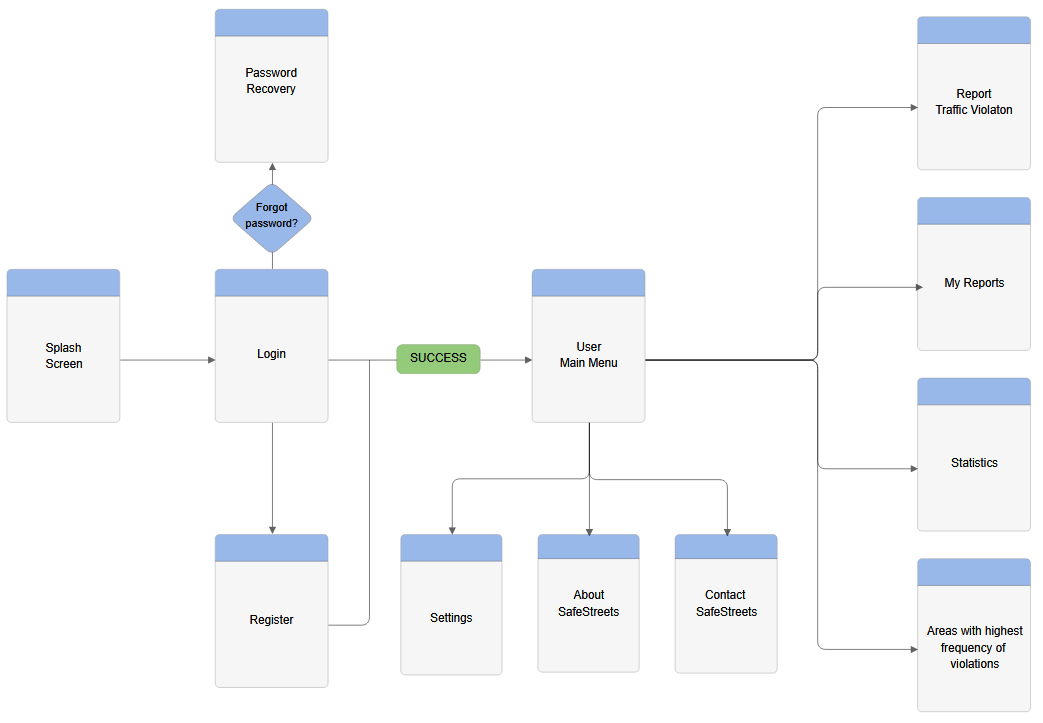
\includegraphics[width=1.25\textwidth,left]{Images/user_experience.png}
        \caption{User UX Diagram}
    \end{figure}
     \begin{figure}[H]
          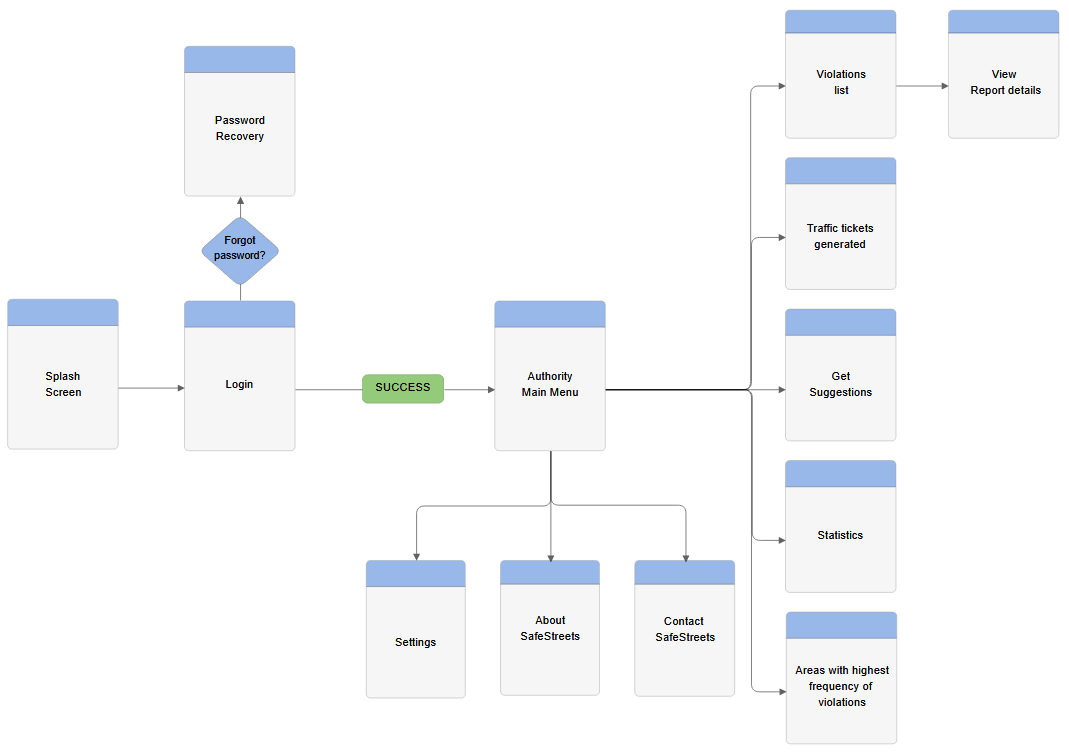
\includegraphics[width=1.25\textwidth,left]{Images/auth_experience.png}
        \caption{Authority UX Diagram}
    \end{figure}
    
   